\subsection{Sequence Diagram}


\begin{figure}[H]
    \centering
    \caption{Sequence Diagram 1}
    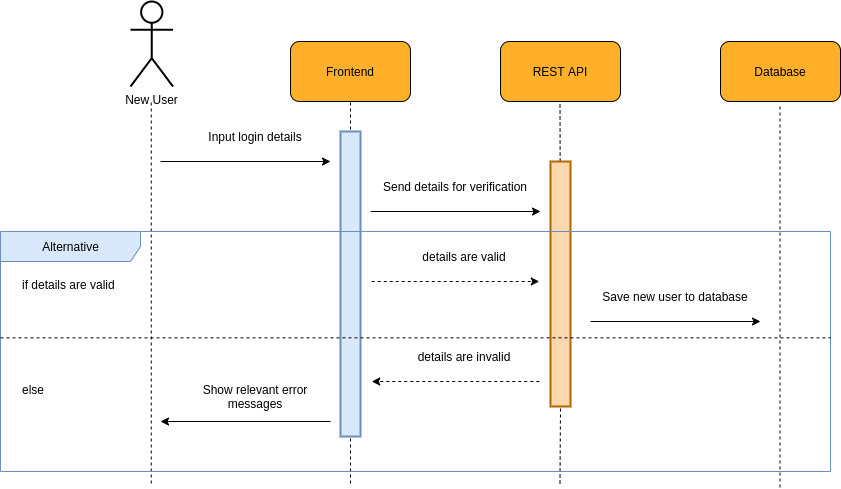
\includegraphics[scale=0.5]{./diagrams/sequence/seq-01.png}
    \label{fig:seq-01}
    
\end{figure}


\begin{figure}[H]
    \centering
    \caption{Sequence Diagram 2}
    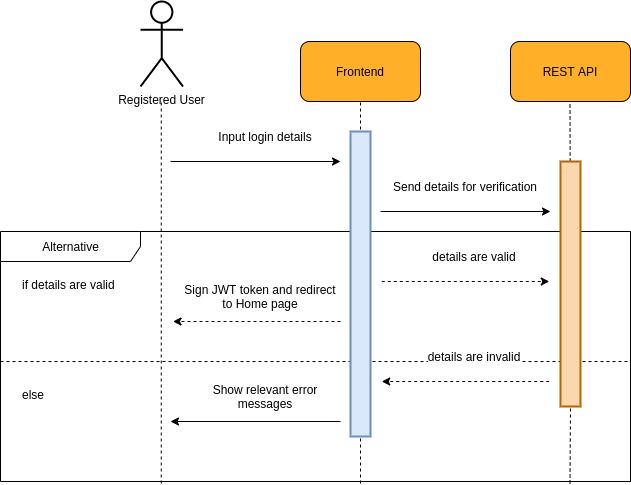
\includegraphics[scale=0.5]{./diagrams/sequence/seq-02.png}
    \label{fig:seq-02}
    
\end{figure}


\begin{figure}[H]
    \centering
    \caption{Sequence Diagram 3}
    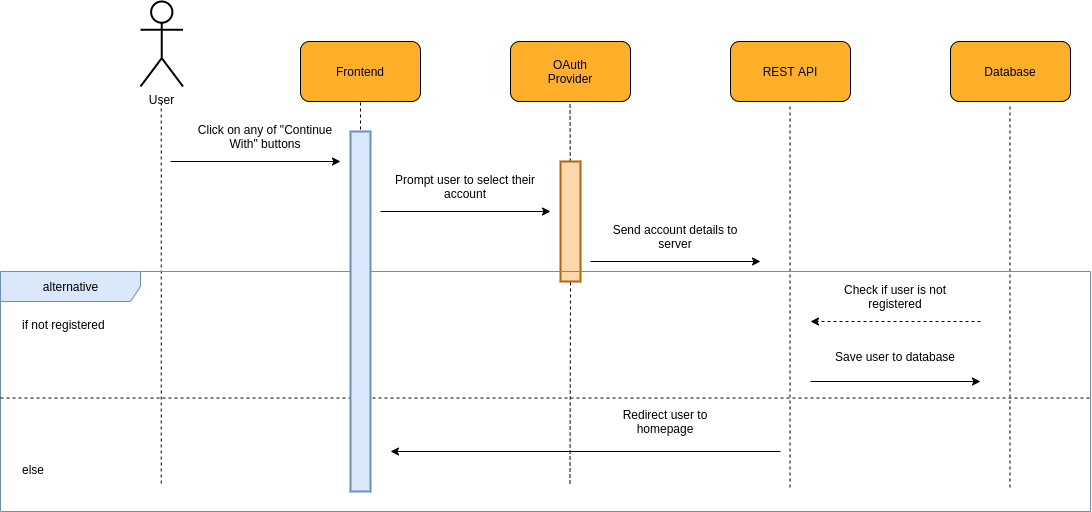
\includegraphics[scale=0.5]{./diagrams/sequence/seq-03.png}
    \label{fig:seq-03}
    
\end{figure}


\begin{figure}[H]
    \centering
    \caption{Sequence Diagram 4}
    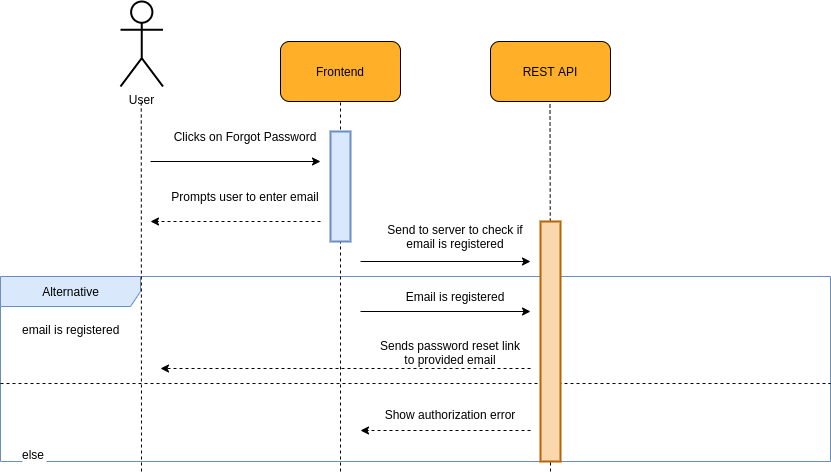
\includegraphics[scale=0.5]{./diagrams/sequence/seq-04.png}
    \label{fig:seq-04}
    
\end{figure}


\begin{figure}[H]
    \centering
    \caption{Sequence Diagram 5}
    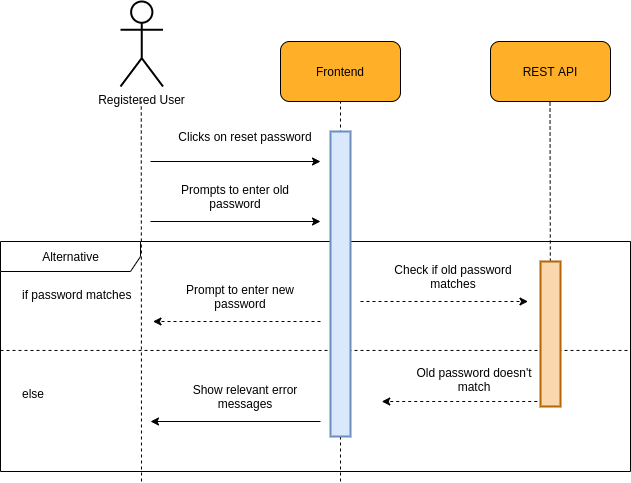
\includegraphics[scale=0.5]{./diagrams/sequence/seq-05.png}
    \label{fig:seq-05}
    
\end{figure}


\begin{figure}[H]
    \centering
    \caption{Sequence Diagram 6}
    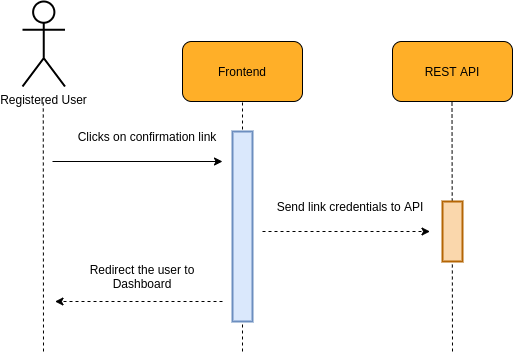
\includegraphics[scale=0.5]{./diagrams/sequence/seq-06.png}
    \label{fig:seq-06}
    
\end{figure}


\begin{figure}[H]
    \centering
    \caption{Sequence Diagram 7}
    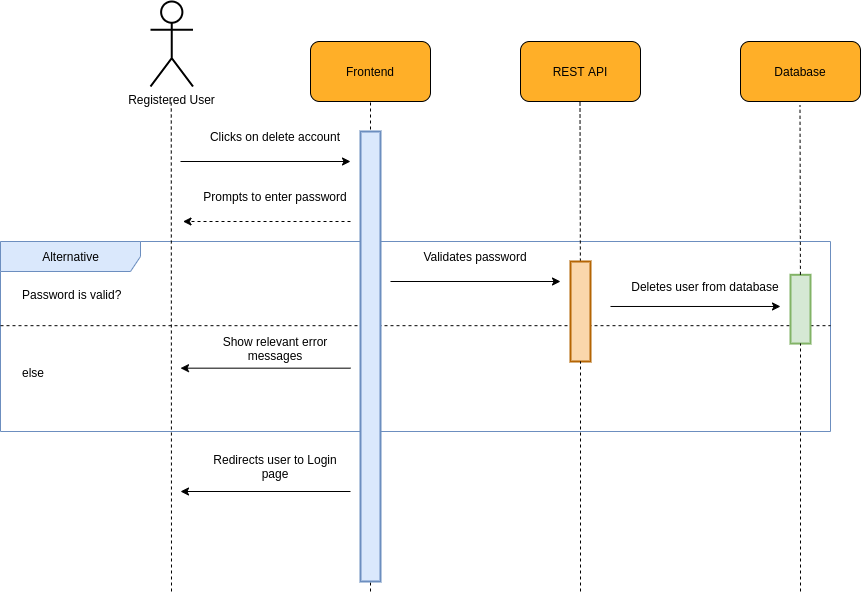
\includegraphics[scale=0.5]{./diagrams/sequence/seq-07.png}
    \label{fig:seq-07}
    
\end{figure}


\begin{figure}[H]
    \centering
    \caption{Sequence Diagram 8}
    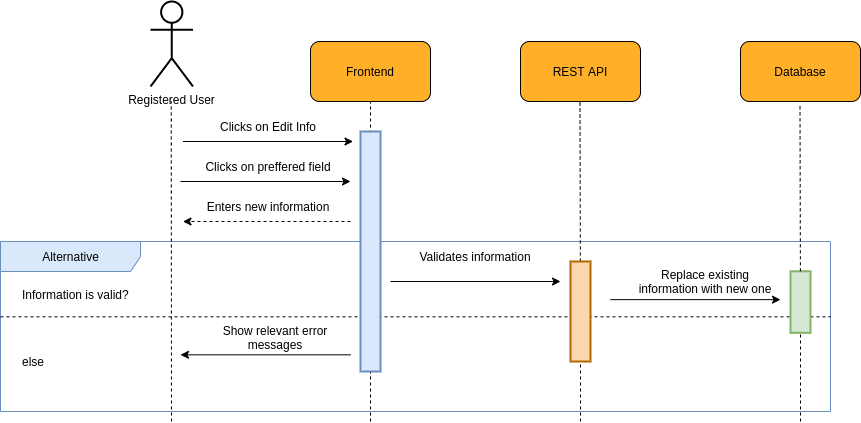
\includegraphics[scale=0.5]{./diagrams/sequence/seq-08.png}
    \label{fig:seq-08}
    
\end{figure}


\begin{figure}[H]
    \centering
    \caption{Sequence Diagram 9}
    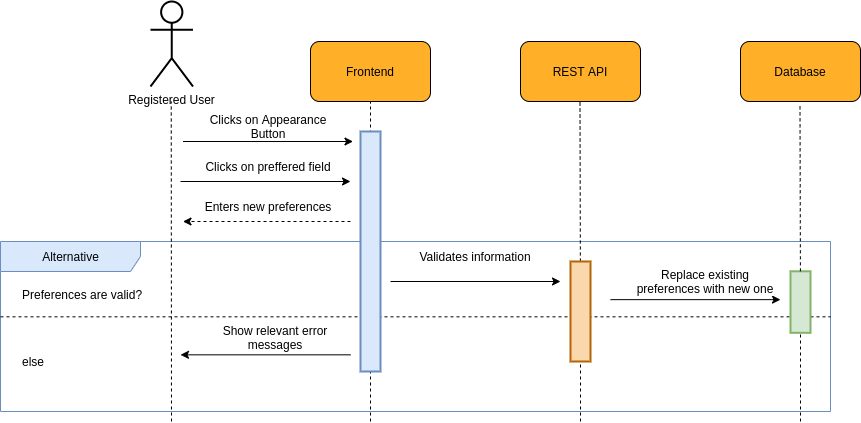
\includegraphics[scale=0.5]{./diagrams/sequence/seq-09.png}
    \label{fig:seq-09}
    
\end{figure}


\begin{figure}[H]
    \centering
    \caption{Sequence Diagram 10}
    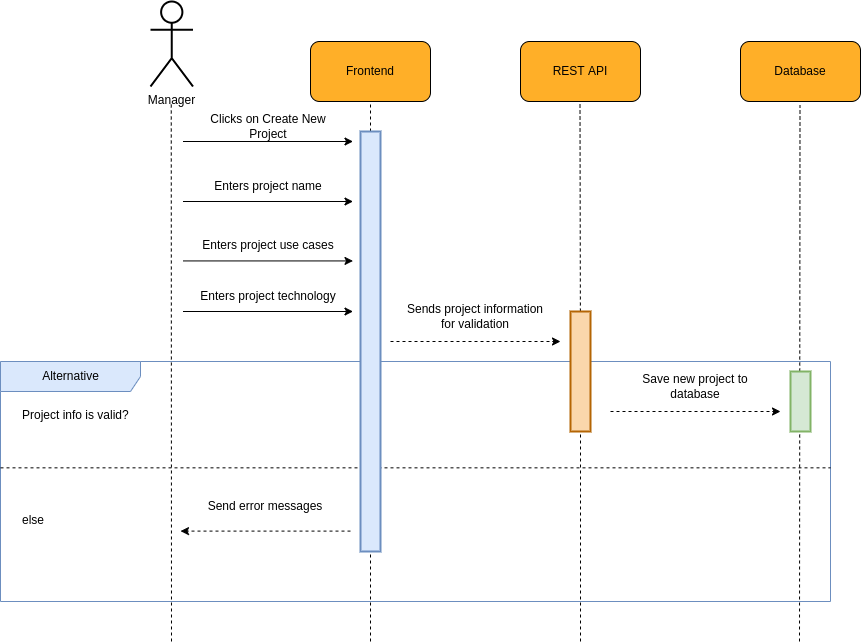
\includegraphics[scale=0.5]{./diagrams/sequence/seq-10.png}
    \label{fig:seq-10}
    
\end{figure}


\begin{figure}[H]
    \centering
    \caption{Sequence Diagram 11}
    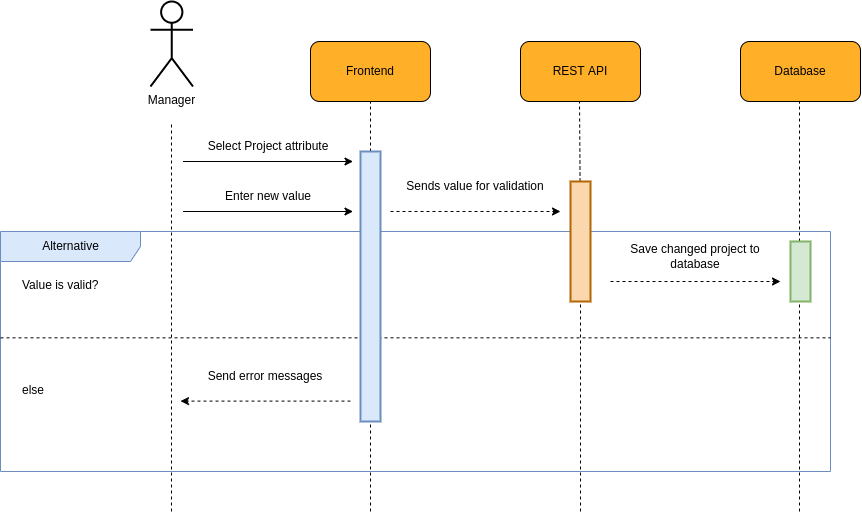
\includegraphics[scale=0.5]{./diagrams/sequence/seq-11.png}
    \label{fig:seq-11}
    
\end{figure}


\begin{figure}[H]
    \centering
    \caption{Sequence Diagram 12}
    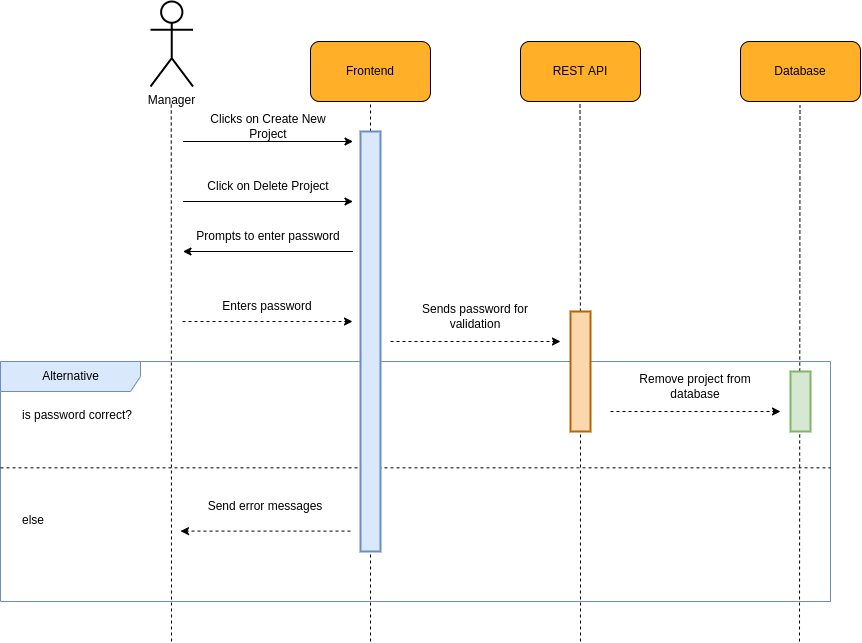
\includegraphics[scale=0.5]{./diagrams/sequence/seq-12.png}
    \label{fig:seq-12}
    
\end{figure}


\begin{figure}[H]
    \centering
    \caption{Sequence Diagram 13}
    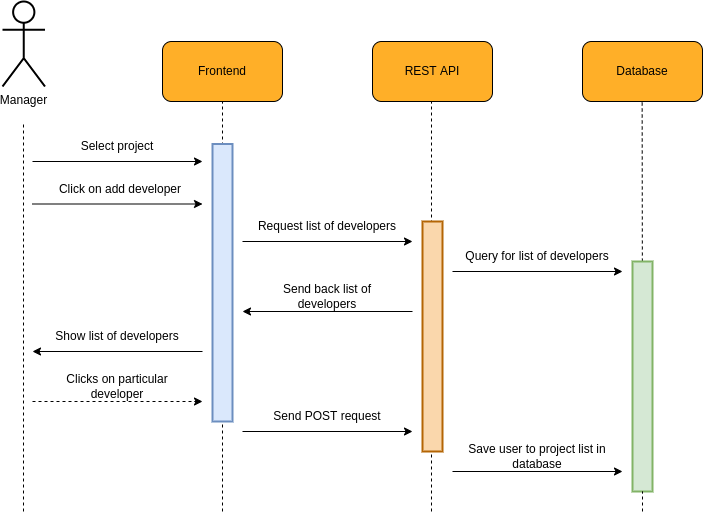
\includegraphics[scale=0.5]{./diagrams/sequence/seq-13.png}
    \label{fig:seq-13}
    
\end{figure}


\begin{figure}[H]
    \centering
    \caption{Sequence Diagram 14}
    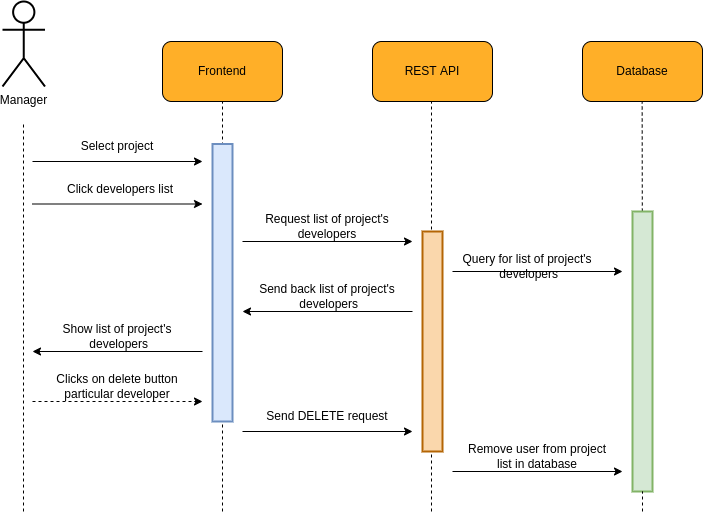
\includegraphics[scale=0.5]{./diagrams/sequence/seq-14.png}
    \label{fig:seq-14}
    
\end{figure}


\begin{figure}[H]
    \centering
    \caption{Sequence Diagram 15}
    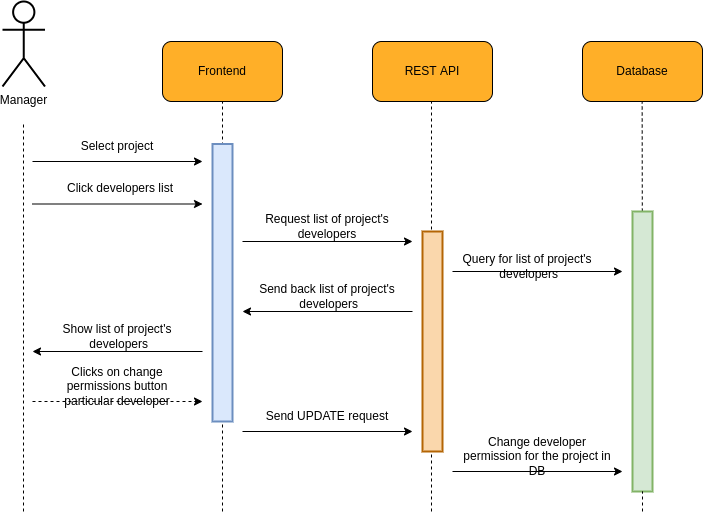
\includegraphics[scale=0.5]{./diagrams/sequence/seq-15.png}
    \label{fig:seq-15}
    
\end{figure}


\begin{figure}[H]
    \centering
    \caption{Sequence Diagram 16}
    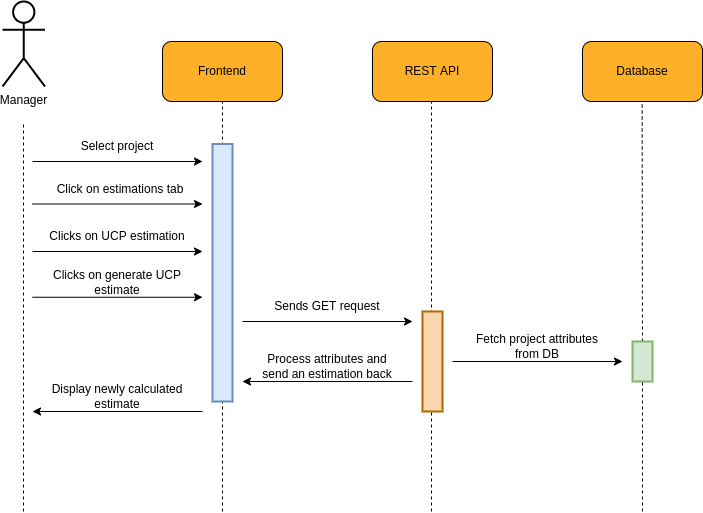
\includegraphics[scale=0.5]{./diagrams/sequence/seq-16.png}
    \label{fig:seq-16}
    
\end{figure}


\begin{figure}[H]
    \centering
    \caption{Sequence Diagram 17}
    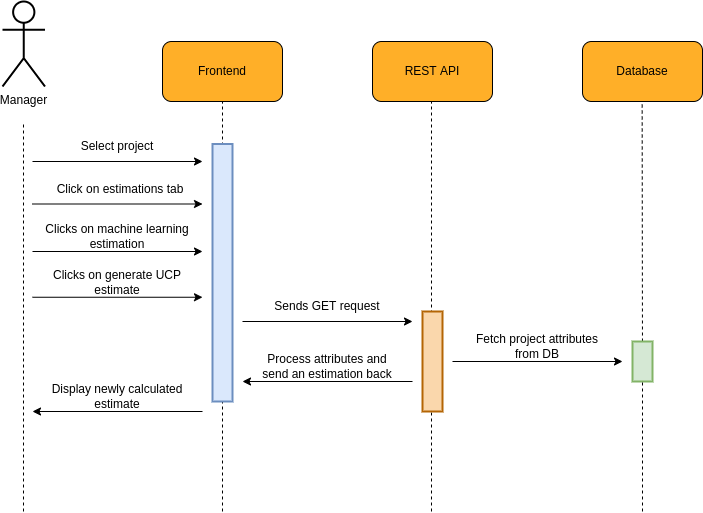
\includegraphics[scale=0.5]{./diagrams/sequence/seq-17.png}
    \label{fig:seq-17}
    
\end{figure}


\begin{figure}[H]
    \centering
    \caption{Sequence Diagram 18}
    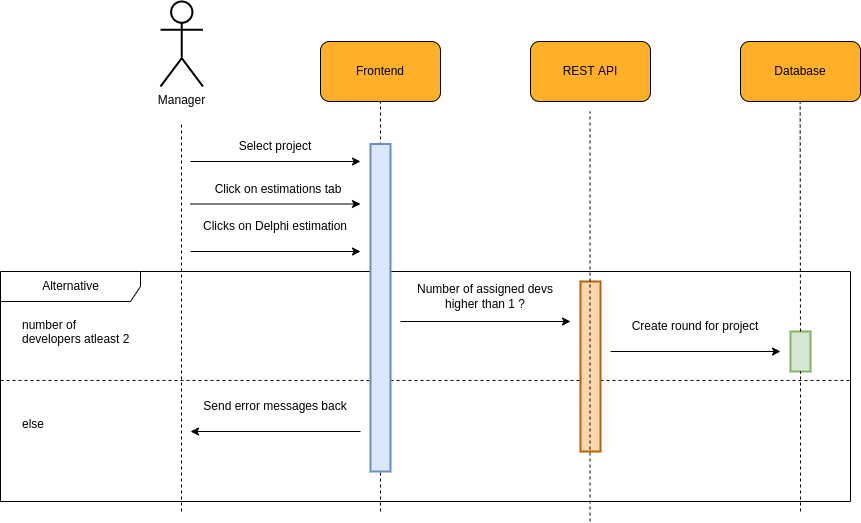
\includegraphics[scale=0.5]{./diagrams/sequence/seq-18.png}
    \label{fig:seq-18}
    
\end{figure}


\begin{figure}[H]
    \centering
    \caption{Sequence Diagram 19}
    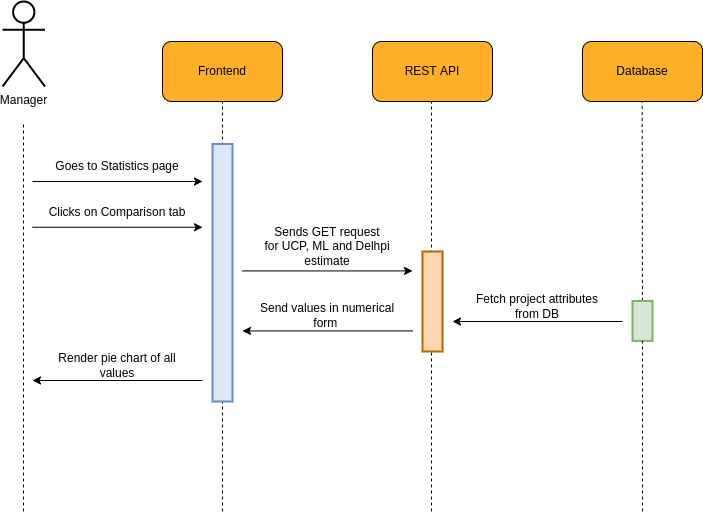
\includegraphics[scale=0.5]{./diagrams/sequence/seq-19.png}
    \label{fig:seq-19}
    
\end{figure}

